\documentclass{article}

% if you need to pass options to natbib, use, e.g.:
% \PassOptionsToPackage{numbers, compress}{natbib}
% before loading nips_2016
%
% to avoid loading the natbib package, add option nonatbib:
%\usepackage[nonatbib]{nips_2016}

%\usepackage{nips}

% to compile a camera-ready version, add the [final] option, e.g.:
\usepackage[final]{nips_2016}

\usepackage[utf8]{inputenc} % allow utf-8 input
\usepackage[T1]{fontenc}    % use 8-bit T1 fonts
\usepackage{hyperref}       % hyperlinks
\usepackage{url}            % simple URL typesetting
\usepackage{booktabs}       % professional-quality tables
\usepackage{amsfonts}       % blackboard math symbols
\usepackage{nicefrac}       % compact symbols for 1/2, etc.
\usepackage{microtype}      % microtypography

\usepackage{amssymb}
\usepackage{mathtools}
\usepackage{latexsym}
\usepackage{amsthm}
\usepackage{enumerate}
\usepackage{epsfig}
\usepackage{graphicx}
\usepackage{color}
\usepackage{float}
\usepackage{subfigure}
\usepackage{amsmath}
\usepackage{MnSymbol}
\usepackage{makeidx}
\usepackage{fancyhdr}
\usepackage{relsize}
\pagestyle{fancy}
\usepackage{lastpage}
\usepackage{url}
\usepackage{mathrsfs}

\newcommand{\F}{\ensuremath{\mathcal F}}
\DeclareMathSymbol{\R}{\mathbin}{AMSb}{"52}
\newcommand{\f}{\ensuremath{\mathcal f}}
\newcommand{\C}{\ensuremath{\mathcal C}}
\newcommand{\M}{\ensuremath{\mathcal M}}
\renewcommand{\H}{\ensuremath{\mathcal H}}
\newcommand{\pisys}{\ensuremath{\mathscr{L}}}
\newcommand{\lsys}[1]{\ensuremath{\lambda \lp #1 \rp}}
\newcommand{\A}{\ensuremath{\mathcal A}}
\newcommand{\E}{\ensuremath{\mathcal E}}
\renewcommand{\L}{\ensuremath{\mathcal L}}
\newcommand{\norm}[1]{\ensuremath{\mathcal \| #1 \|}}
\newcommand{\Exp}[1]{\ensuremath{\mathbb{E} \lb #1 \rb}}
\newcommand{\condExp}[2]{\ensuremath{\mathbb{E} \lb #1 | #2 \rb}}
\newcommand{\lp}{\ensuremath{\left(}}
\newcommand{\rp}{\ensuremath{\right)}}
\newcommand{\lb}{\ensuremath{\left[}}
\newcommand{\rb}{\ensuremath{\right]}}
\newcommand{\B}[1]{\ensuremath{\mathcal B\lp #1 \rp}}
\newcommand{\Pset}[1]{\ensuremath{\mathcal P\lp #1 \rp}}
\newcommand{\siga}[1]{\ensuremath{\sigma\lp #1 \rp}}
\newcommand{\Xrv}[1]{\ensuremath{X\lp #1 \rp}}
\newcommand{\Xrvi}[1]{\ensuremath{X \inv \lp #1 \rp}}
\newcommand{\Yrv}[1]{\ensuremath{Y\lp #1 \rp}}
\newcommand{\Prob}[1]{\ensuremath{\Pb\lp #1 \rp}}
\newcommand{\inv}{\ensuremath{^{-1}}}
\newcommand{\iprod}[2]{\ensuremath{\llangle #1, #2 \rrangle}}
\newcommand{\twopartdef}[4]
{
	\left\{
		\begin{array}{ll}
			#1 & \mbox{if } #2 \\
			#3 & \mbox{if } #4
		\end{array}
	\right.
}
\newcommand\independent{\protect\mathpalette{\protect\independenT}{\perp}}
\def\independenT#1#2{\mathrel{\rlap{$#1#2$}\mkern2mu{#1#2}}}

\title{Prior Formulation for Gaussian Process Hyperparameters}

% The \author macro works with any number of authors. There are two
% commands used to separate the names and addresses of multiple
% authors: \And and \AND.
%
% Using \And between authors leaves it to LaTeX to determine where to
% break the lines. Using \AND forces a line break at that point. So,
% if LaTeX puts 3 of 4 authors names on the first line, and the last
% on the second line, try using \AND instead of \And before the third
% author name.

\author{
  Rob Trangucci \\
  Applied Statistics Center\\
  Columbia University\\
  New York, NY 10027 \\
  \texttt{rnt2101@columbia.edu} \\
  \and
  Michael Betancourt \\
  Applied Statistics Center \\
  Columbia University \\
  New York, NY 10027 \\
  \texttt{betanalpha@gmail.com} \\
}

\begin{document}
% \nipsfinalcopy is no longer used

\maketitle

\begin{abstract}
  Gaussian processes are measures over functions, and as such, can be used as a
  rich prior for latent functions in Bayesian statistical models. However, the
  joint posterior density of the length scale and marginal variance
  hyperparameters in stationary kernels like the exponentiated quadratic and
	M\'{a}tern is often weakly informed by the data because of the extreme
  flexibility of Gaussian process priors. We develop a principled approach for
  specifying weakly informative priors for length scale hyperparameters that impose
  soft constraints on the space of functions represented by the Gaussian
  process prior.
\end{abstract}


\section{Introduction}

As noted by many authors (\citet{flaxman2015fast},
\citet{stein2012interpolation}, \citet{rasmussen2005gaussian},
\citet{fuglstad2015interpretable}), learning hyperparameters in Gaussian
process (GP) kernels is notoriously hard. The preponderance of literature has
focused estimating hyperparameters using marginal maximum likelihood for point
estimation (\citet{stein2012interpolation}, \citet{rasmussen2005gaussian}, \citet{warnes1987problems}), and
the asymptotic properties of posterior conditional mean functions in GP
regressions (\citet{seeger2008information}, \citet{stein2012interpolation},
\citet{rasmussen2005gaussian}, \citet{williams2000upper}). As applied
statisticians, we face datasets with finitely many observations. As such there
will be many sets of hyperparameters that are consistent with our data; picking
any one set of them will lead to overfitting and poor out-of-sample
predictions. Instead, we would advocate placing priors over hyperparameters and
integrate over our uncertainty when making predictions for new data. For
maximum flexibility in model building, we would like to select weakly
informative priors, run our MCMC chains to convergence, and calculate posterior
expectations for our estimands of interest. 

Unfortunately, poorly-chosen weakly informative priors
can yield large posterior intervals for hyperparameters and lead to wide
posterior predictive intervals when data are not informative about model
parameters (\citet{fuglstad2015interpretable}). Thus, we need a better
understanding of how weakly informative priors interact with the likelihood
under a Gaussian process prior.

In order to gain insight into the empirical behavior of different priors, we
explore how efficiently 4 weakly informative priors can extract known
parameters in 12 different data generating processes, using techniques from
\citet{cook2012validation}. We chose to study the deliberately simple 1-D
Gaussian process regression model in order to elucidate the pathologies
inherent in posterior inference over kernel hyperparameters. Additionally, we
aspire to develop a coherent framework to choose weakly informative priors that
can effectively regularize nonidentifiabilities. It is important to note that
GPs in higher-dimensional spaces will likely display different idiosyncracies
than observed in the low-dimensional setting and these warrant further study.

In section \ref{background} we define the 1-D Gaussian process regression setting,
the hyperparameters of interest, and the mathematical basis for the manifestations
of weak identifiability in kernel hyperparameters. In section \ref{experiment}, we 
outline the experimental set up, and in section \ref{results} we discuss the results 
of our experiments. Stan code is presented in the appendix.

\section{Background} \label{background}

\subsection{Gaussian processes regression}

The typical regression setting for observed univariate data, as presented in \citet{flaxman2015fast},

$y_i \in \R, x_i \in \R^M\, i \in {1,\dots,n}$:

\begin{align*}
  \theta & \sim g(\phi) \\
  f(x) & \sim \text{GP}\lp \mu(x),
  K_\theta(x, x) \rp \\
  y_i & \sim \mathcal{N}\lp f(x_i), \delta \rp \forall i \\
\end{align*}

where $\text{GP}$ is a stochastic process from which finite-sample realizations are
multivariate Gaussian, and which is completely specified its mean vector $\mu$
and its covariance matrix $K_\theta(x, x)$. The $i, j$ th
element of $K_\theta(x, x)$:

\begin{align*}
  \text{cov}(f(x_i), f(x_j)) = k(x_i, x_j | \theta) 
\end{align*}

We focus on the squared exponential kernel, where $\theta$ comprises
two hyperparameters, $\ell$, the length-scale, and $\alpha$, the marginal
standard deviation:

\begin{align} \label{kern}
  k(x_i, x_j | \alpha, \ell) = \alpha^2 
\exp \left(
	- \dfrac{1}{2\ell^2} (x_{i} - x_{j})^2
\right)
\end{align}

With $\ell$ and $\alpha$ fixed, inference of $f(x | \, \mathbf{y}, \theta)$ is
straightforward, with $f$ and $\mathbf{y}$ jointly normally distributed:
%put arrow above y and x to indicate vector of x and y $$:

\begin{align*} \begin{pmatrix} f\\ \mathbf{y} \\ \end{pmatrix} \sim
\mathcal{N} \lp \begin{pmatrix} \mathbf{0} \\ \mathbf{0} \end{pmatrix} ,\,\,
  \begin{pmatrix} K_\theta &
  K_\theta  \\ K_\theta &
  K_\theta + \delta ^ 2 \mathbf{I}\\ \end{pmatrix} \rp
\end{align*}

We can derive $p(f | \mathbf{y})$ from the properties of the conditional normal
distribution: 

\begin{align*}
  f \sim
  \mathcal{N}(K_\theta  (K_\theta + \delta ^ 2 \mathbf{I})^{-1}\mathbf{y},  
  K_\theta - K_\theta (K_\theta + \delta ^ 2 \mathbf{I})^{-1}K_\theta)
\end{align*}

Out-of-sample predictions are generated similarly:

\begin{align*} 
  \mathbf{\tilde{y}} \sim
  \mathcal{N}(&K_\theta(\mathbf{\tilde{x}},\mathbf{x}) (K_\theta(\mathbf{x},\mathbf{x}) +
  \delta ^ 2 \mathbf{I})^{-1}\mathbf{y},  
   \\ & K_\theta(\mathbf{\tilde{x}},\mathbf{\tilde{x}}) -K_\theta(\mathbf{\tilde{x}},\mathbf{x}) (K_\theta(\mathbf{x},\mathbf{x}) + \delta ^ 2 \mathbf{I})^{-1}K_\theta(\mathbf{x},\mathbf{\tilde{x}}) + \delta ^ 2 \mathbf{I})
\end{align*}

\begin{figure} \label{prior-lat-draws}
  \makebox[\textwidth]{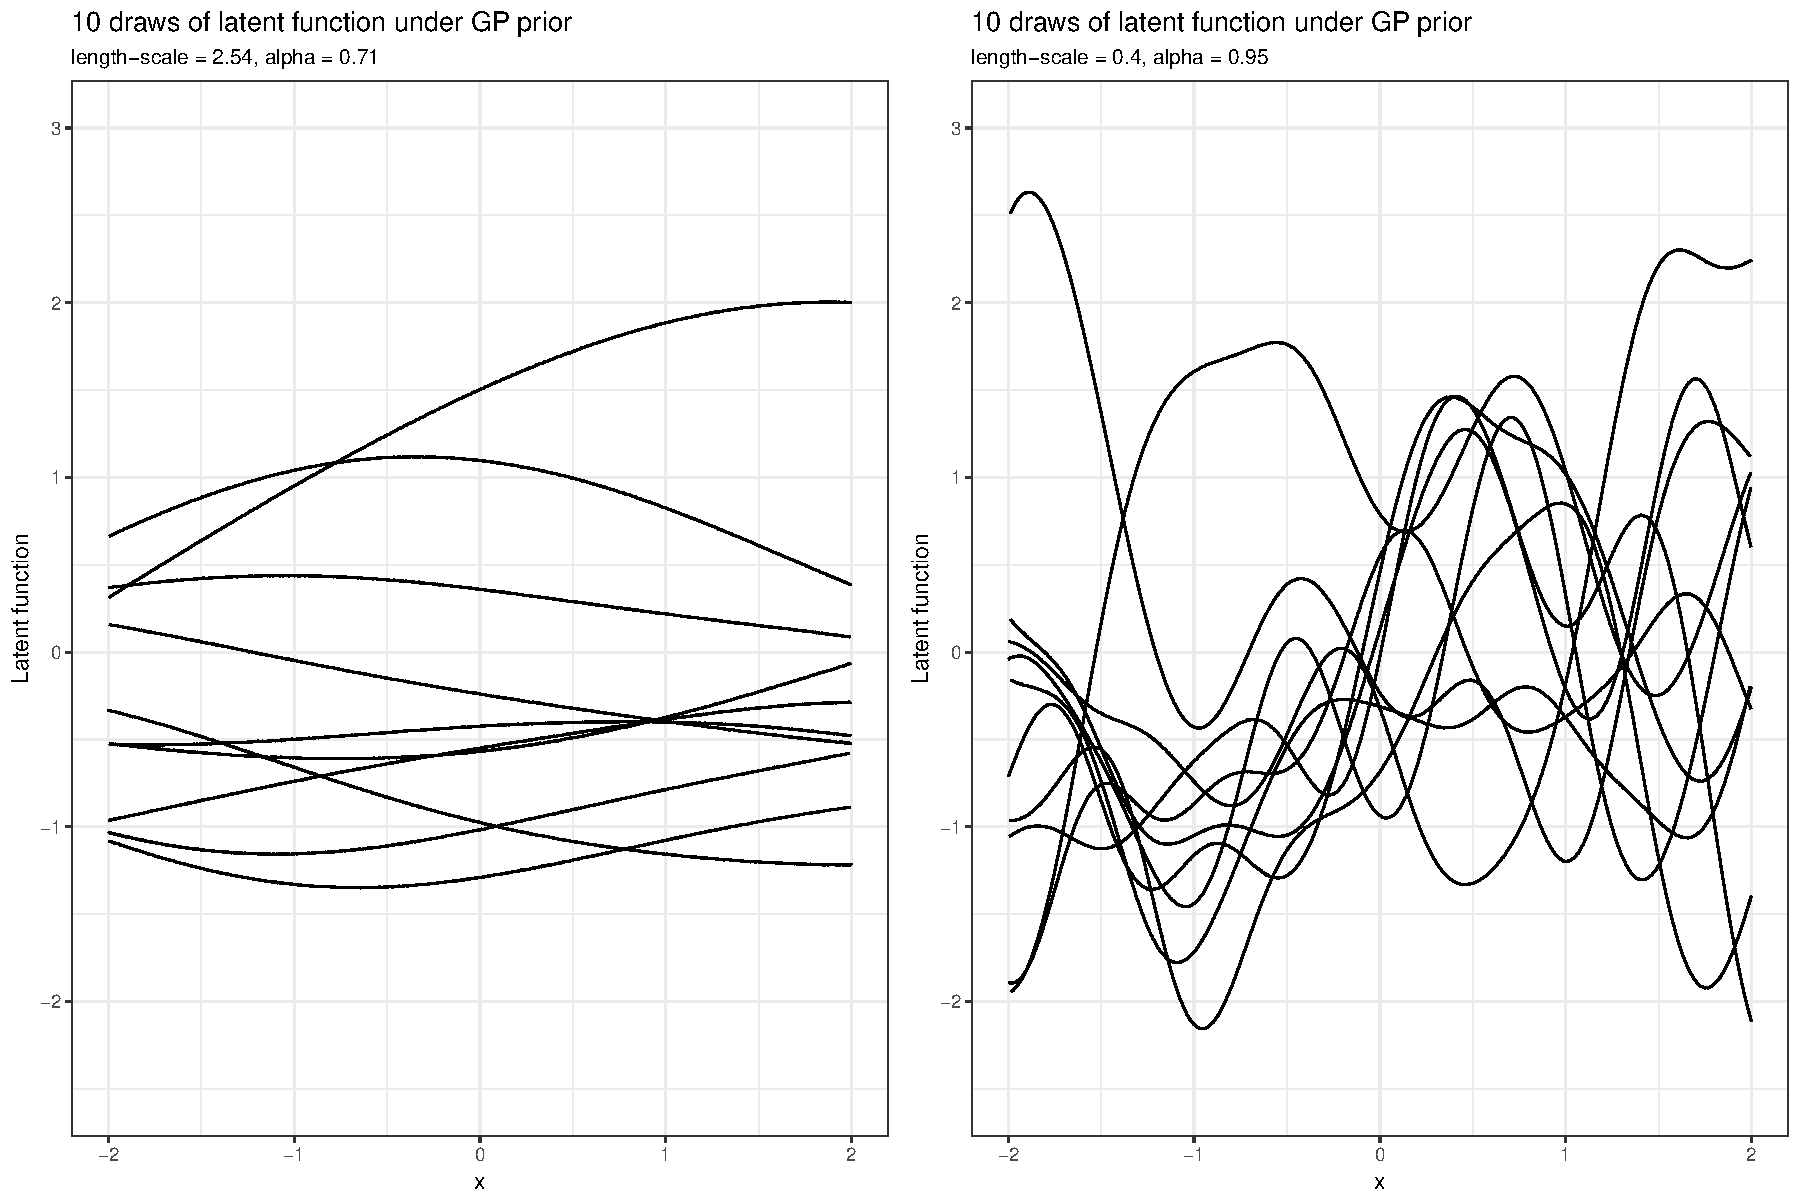
\includegraphics[width=\textwidth,height=50mm]{plots/latent_draws_comparison.pdf}}
  \caption{Parameters which lead to expected zero crossings of 1/2 on left and 3.16 crossings on right} \label{prior-lat-draws}
\end{figure}

However, if we want to infer $\theta$ from the data we will need to take our
uncertainty in $\theta$ into account. We can see that both $\ell$ and $\alpha$
will impact our predictions for $\tilde{\mathbf{y}}$. $\alpha^2$ controls the
marginal variance of the stochastic process. For a fixed noise variance,
$\delta^2$, increasing the marginal variance of the stochastic process
increases the signal-to-noise ratio, $\alpha^2 / \delta^2$ (SN). $\ell$
controls the process's nonlinearity. Figure 1 shows the
difference between draws from a GP prior with a large $\ell$ and draws from a
GP prior with a small $\ell$.


Naturally, $\ell$ and $\alpha$ also control observable statistics of the
GP like the expected number of crossings of $f(x)$ on the interval $[0,
T]$ at level $u$, $\Exp{C_u}$. \citet{cramer2004stationary} show that $\Exp{C_u}$:

\begin{align*} 
  \Exp{C_u | \theta} = \dfrac{T}{\pi} 
\sqrt{-\dfrac{k_\theta^{\prime \prime}(0)}{k_\theta(0)}}
  \text{exp}\left(-\dfrac{u^2}{2k_\theta(0)}\right)
\end{align*} 

For the $\Exp{C_u | \theta}$ exponentiated quadratic kernel:

\begin{align*} 
  \Exp{C_u | \alpha, \ell} = \dfrac{T}{\pi \ell}\text{exp}\left(-\dfrac{u^2}{2 \alpha ^ 2} \right)
\end{align*} 

We can see that at $u = 0$, we are left with $\Exp{C_u | \alpha, \ell} = T / \pi \ell$.  

However, at $u \neq 0$ $\alpha$ and $\ell$ are conflated in $\Exp{C_u | \alpha,
\ell}$.  This is an inevitability of the parameterization of the exponentiated
quadratic kernel, and this feature of GPs can lead to problems when 
estimating $\alpha$ and $\ell$ from data.

\subsection{Identifiability}

In order to estimate unknown parameters in a parametric statistical model using
maximum likelihood, the likelihood must change its value when evaluated at
distinct values of the parameters. If that is not the case, then the parameter
is said to be unidentifiable. Intuitively, if two values of a parameter
generate two identical datasets, how can we expect to extract information about
that parameter from the data? Formally, we have a vector-valued random variable
$Z \in \R^L$, with a family of densities, $p(z | \gamma)$, where $\gamma$ are
unknown in $\R^S$. If $\gamma_1, \gamma_2 \in \R^S$ and 

\begin{align*}
  p(z | \gamma_1) = p(z | \gamma_2) \forall z \in \R^L
\end{align*}

then we can say that $\gamma$ is unidentified. A example of unidentifiablity is
a normal density for $z \in \R^1$ parameterized with two location parameters,
$\beta$ and $\psi$. The likelihood is invariant to an additive shift $c$ to
$\beta$ and a negative shift $c$ to $\psi$ (or vice-versa). Thus, the
likelihood does not have a maximum with respect to $\beta$ and $\psi$. Note
that this example is pathological, and can be alleviated by using a single
location parameter.  Nevertheless, it is instructive as to the flavor of
identifiability problems which can occur when the data do not constrain our
estimate of the parameter. The classical definition of unidentifiable provided
above must hold for all $z$. 

For Bayesian inference, identifiability is more nuanced. If we are faced with a
classically unidentified parameter like above, we can put proper priors on
$\beta$ and $\psi$ and sample from the posterior, as shown in
\cite{xie2004note}. In some sense, any set of priors will do because the
parameters cannot be informed by any dataset. The posterior estimates
are only possible through constraining the parameters using priors. 

However, the Gaussian process parameterized with an isotropic kernel like
\ref{kern} lies on the spectrum between classically unidentified and
classically identified. If the data do not adequately constrain the parameters
$\alpha$ and $\ell$, we need to add additional structure to the posterior in
the form of priors that limit probability mass in the tail. If we do not
we can get behavior that appears like classical unidentifiability in the 
tail of the distribution: a flat log-posterior along $\ell$'s axis. 

We use the term ``weak identifiability'' to refer to a pathology wherein a
subset of its parameters exhibit behavior consistent with classical
unidentifiability in certain regions of parameter space. This occurs when the
data are not informative about this subset of parameters.  We avoid a formal
definition because this is an open research question and not the focus of this
paper.

\subsection{Weak identifiability in GPs}

\citet{rasmussen2005gaussian} show that a kernel $k(\boldsymbol{\tau})$ can
represented in the frequency domain by its Fourier transform:

\begin{align*}
  S(\mathbf{s}) = \int k(\mathbf{\tau}) \exp \left( -2 \pi i \mathbf{s}  \boldsymbol{\tau} \right) d\mathbf{s}
\end{align*}

The power spectrum for the exponentiate quadratic kernel can be derived analytically:

\begin{align*} 
  S(s) \propto \alpha^2 \ell
   \exp \left(
  - 2 \pi^2 \ell^2 s^2
\right)
\end{align*} 

This can be interpreted as the weight the kernel gives to an eigenfunction with
frequency $s$. Thus, for large $\ell$ the kernel gives more weight to low
frequency eigenfunctions and less weight to high-frequencye eigenfunctions. The 
total power of the spectrum 

We see problems with the spectrum of the kernel because both the $\alpha ^ 2$
term and the $\ell$ term scale the density $\exp \left(- 2 \pi^2 \ell^2 s^2
\right)$ term. In settings with sparse data and a low frequency signal,
increasing $\ell$ will force $S(s)$ to allocate more power to low frequency
signals at the expense of high frequency. Increasing $\alpha$ will allocate
more power to all frequencies, but because the data are low-frequency and
sparse, we will not have enough resolution to distinguish between an increase
in $\alpha$ or an increase in $\ell$. We can see that we will have the same
problem with high frequency signals and sparse data. As $\ell$ decreases,
we allocate more power to high-frequency functions at the expense of 
low-frequency functions. We can decrease $\alpha$ in order to decrease
the power allocated to all frequencies, but the sparsity of the data
necessarily means we will not be able to learn the fine-resolution
structure of the spectral density.

Note that the intuition provided above does not fit the definition of 
classical unidentifiability; the spectral density certainly does change
values for two distinct sets of hyperparameters. However, sparse data
may not provide enough constraint to infer the hyperparameters effectively.

Our intuition says that the multiplicative term might lead to positive
posterior correlation between $\alpha$ and $\ell$. However, it is not clear
whether using strong independent prior information will mitigate this posterior
correlation, nor is it clear how weak priors over $\ell$ will manifest
themselves in posteriors over $\alpha$. 

Turning to equation \ref{kern} again, we can see that the limiting behavior of
the GP as $\ell \rightarrow \infty$ and $\alpha \rightarrow 0$ each lead to the
constant function. We can also see that $\ell \rightarrow 0$ will conflate
inferences in $\delta$.  Note that as $\ell \rightarrow 0$ $\Exp{C_u | \alpha,
\ell}$ diverges.

\section{Experiment} \label{experiment}

We investigate the properties of posterior inferences under several prior
formulations by generating 100 datasets for 12 data generating processes and
subsequently inferring $\alpha$, $\ell$, and $\delta$ by using Stan.

\subsection{Priors}

Limiting behavior of GPs is an important driver of weak identifiability, so we
decided to choose priors that differed in probability mass near zero and mass
in the tails of the densities, but that were similar in mass at other regions
of support. Thus, we calibrate our choices of priors for $\ell$ by fixing the
amount of probability mass between 0 and 1 for each prior at $\sim60\%$ but by
varying the priors' mass near zero and by varying the priors' tail heaviness.

This yields 4 priors: $\text{Gamma}(2, 2)$, $\text{Half-Cauchy}(0, 0.7)$,
$\text{Half-Normal}(0, 1.2)$, $\text{Weibull}(2, 1)$

\begin{figure}[t] 
  \makebox[\textwidth]{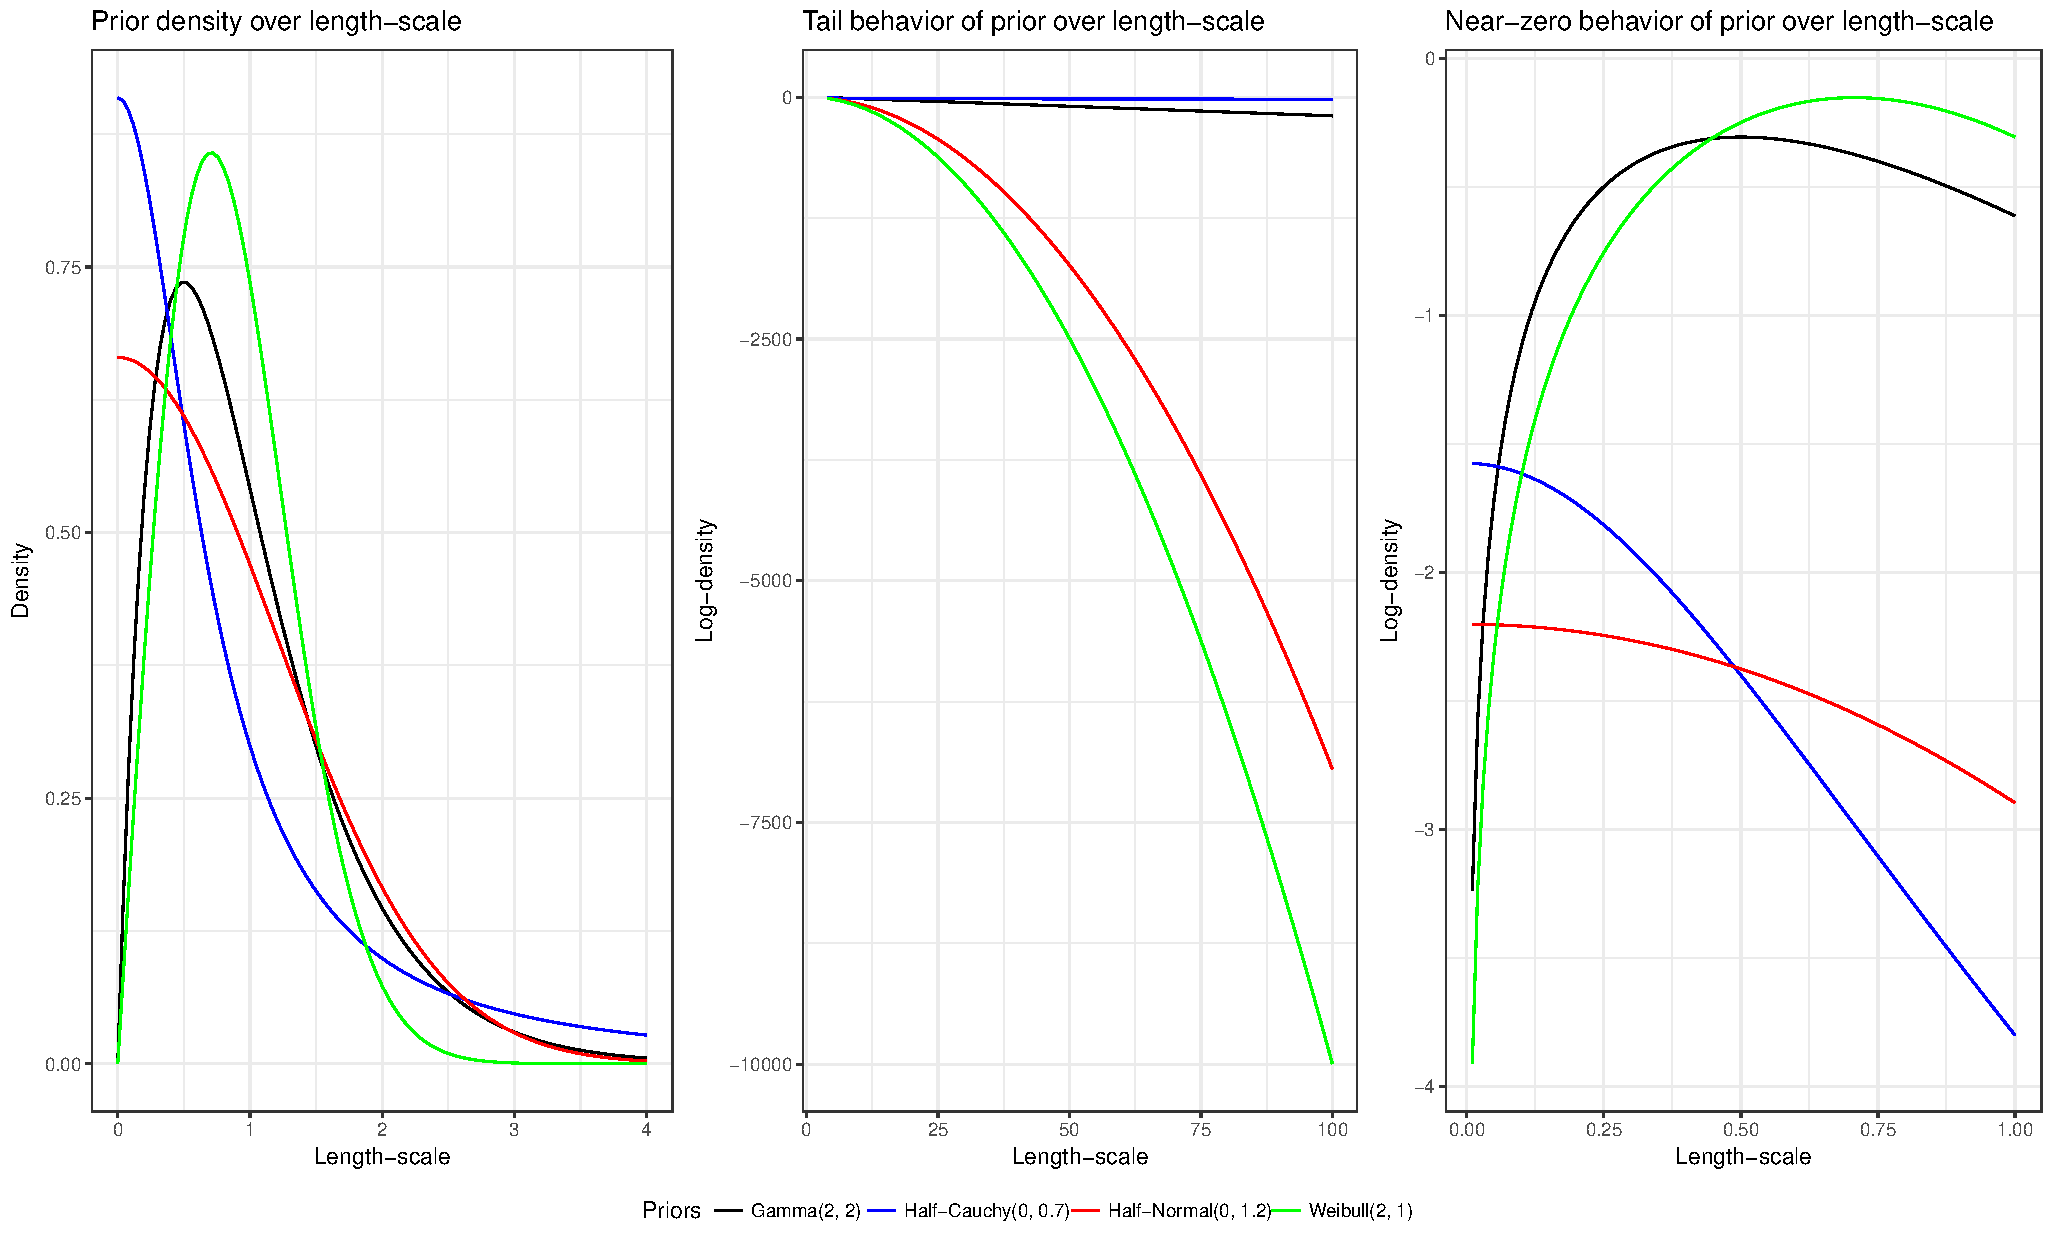
\includegraphics[width=\textwidth,height=50mm]{plots/prior_0_4_chart.pdf}}
  \caption{Priors over $\ell$ (length-scale)} \label{prior_plot}
\end{figure}

The $\text{Half-Cauchy}(0, 0.7)$ has the most mass at zero, and the most tail
mass. $\text{Gamma}(2, 2)$ has a heavy tail, but much lighter mass near zero
(in fact, it has zero mass exactly at zero, and thus is a zero-avoiding prior
\citet{gelman2014bayesian}). The $\text{Half-Normal}(0, 1.2)$ has a much
lighter tail than either the $\text{Half-Cauchy}(0, 0.7)$ or the
$\text{Gamma}(2, 2)$, but still has quite a bit of mass near zero.
$\text{Weibull}(2, 1)$ has about as much mass near zero as $\text{Gamma}(2, 2)$
but its tails are lighter than $\text{Half-Normal}(0, 1.2)$.

We fix our priors for $\alpha$ and $\delta$ as $\text{Half-Normal}(0, 1)$. We
decided not to vary the parameters of $\alpha$ or $\delta$ because we believe
that by applying well-constructed priors to $\ell$ we can mitigate problems
in estimating $\alpha$. 

\subsection{Datasets}

We simulated 100 datasets of 500 uniformly sampled data points on the domain
from $[-2, 2]$ from a Gaussian process regression for 12 sets of parameters.
The data generating processes vary in the severity of the nonlinearity in the
Gaussian process prior, induced by scaling $\ell$ from near $0.04$ to $2.54$.
We then generated two sets of 100 replicated datasets at each $\ell$, one set
which had a signal-to-noise ratio $\alpha ^ 2/ \delta ^ 2$ (SN) of $1$ and one
set which had a signal-to-noise ratio of $10$. The marginal variance $\alpha ^
2 + \delta ^ 2$ was fixed at 1 for each parameter set. The full data set
parameters are below:

\begin{table}[ht]
\centering
\begin{tabular}{rrrrrr}
  \hline
  & $\alpha$ & $\delta$ & SN & $\ell$ & $\Exp{C_0}$ \\ 
  \hline
1 & 0.71 & 0.71 & 1.00 & 2.54 & 0.50 \\ 
  2 & 0.95 & 0.30 & 10.00 & 2.54 & 0.50 \\ 
  3 & 0.71 & 0.71 & 1.00 & 1.27 & 1.00 \\ 
  4 & 0.95 & 0.30 & 10.00 & 1.27 & 1.00 \\ 
  5 & 0.71 & 0.71 & 1.00 & 0.64 & 2.00 \\ 
  6 & 0.95 & 0.30 & 10.00 & 0.64 & 2.00 \\ 
  7 & 0.71 & 0.71 & 1.00 & 0.40 & 3.16 \\ 
  8 & 0.95 & 0.30 & 10.00 & 0.40 & 3.16 \\ 
  9 & 0.71 & 0.71 & 1.00 & 0.13 & 10.00 \\ 
  10 & 0.95 & 0.30 & 10.00 & 0.13 & 10.00 \\ 
  11 & 0.71 & 0.71 & 1.00 & 0.04 & 31.62 \\ 
  12 & 0.95 & 0.30 & 10.00 & 0.04 & 31.62 \\ 
   \hline
\end{tabular}
\end{table}

\subsection{Inference}

We ran Stan on the command line (\citet{cmdstan}) for 1000 warmup and 1000
post-warmup iterations with 4 MCMC chains. All simulations run achieved
$\hat{R}$ < 1.05 for all parameters and achieved an acceptable effective sample
size, as suggested by \citet{gelman2014bayesian}.

\section{Results} \label{results}

We confirm our intuition that in settings with sparse data the tails of the
posterior distribution under heavy-tailed priors like the Cauchy are fat and
can lead to biased inferences. An illuminating example that arose from the
setting in which the signal-to-noise ratio was 1 and $\ell$ was set to 2.54 is
worth highlighting.

The data and the latent mean functions are nearly constant across the $[-2,2]$
interval, as shown in figure $\ref{gp_set_3}$. Our inferences for $\ell$ and $\alpha$
are plotted in figure \ref{gp_set_3_len}. The Cauchy model has clear problems ruling
out the constant function in its posterior. This has implications for the 
posterior predictive mean distribution, which was biased sharply towards
constant functions, as can be seen in figure \ref{gp_set_3_post_pred_cauchy}. The
posterior predictive mean distribution from the $\text{Half-Normal}(0, 1.2)$
prior over $\ell$ is better, though we can see the model still having trouble
distinguishing the true latent mean function. This is to be expected in settings
where the signal-to-noise ratio is low and the data are not informative.

\begin{figure}[h]
  \centering
  \makebox[\textwidth]{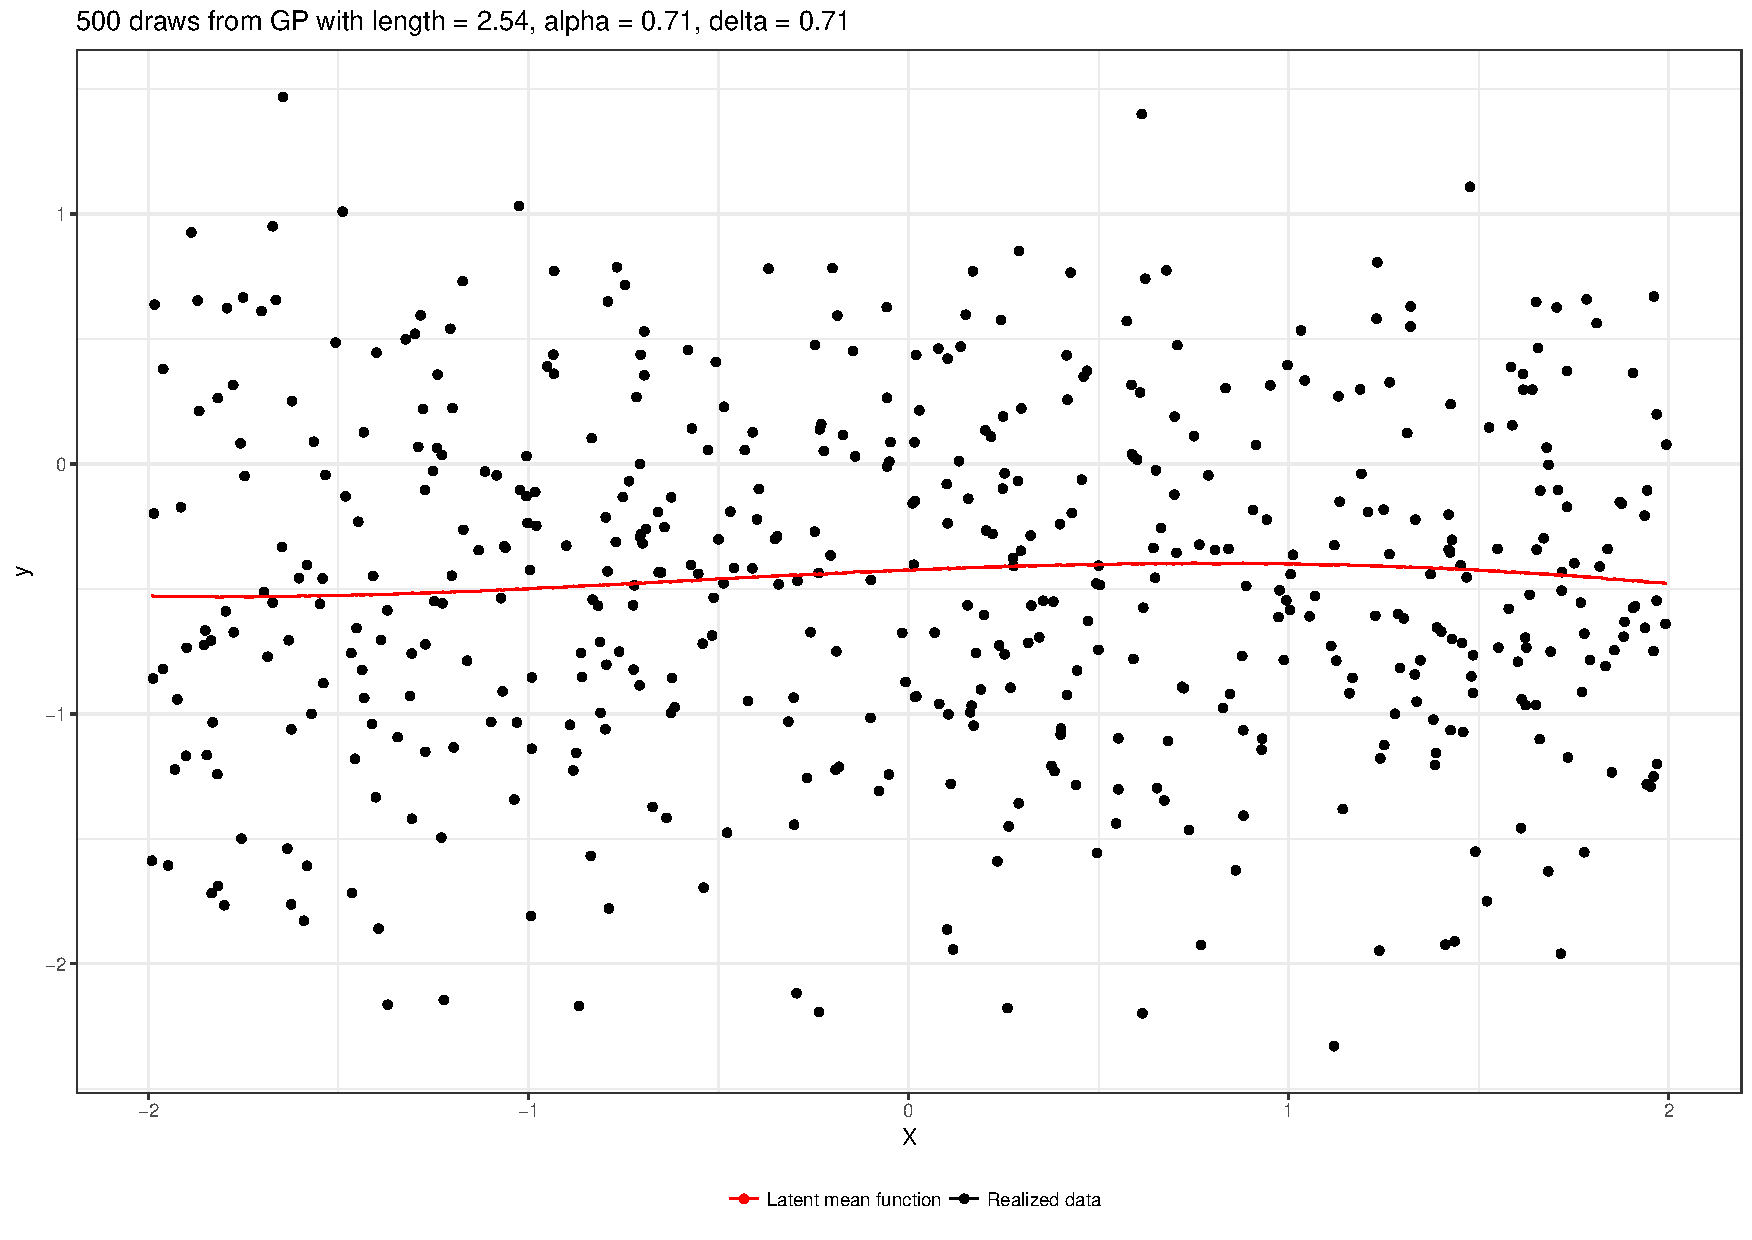
\includegraphics[width=\textwidth]{plots/dset_3_dgp.pdf}}
  \caption{Synthetic dataset with nearly constant latent function and high noise} \label{gp_set_3}
\end{figure}

\begin{figure}[h]
  \centering
  \makebox[\textwidth]{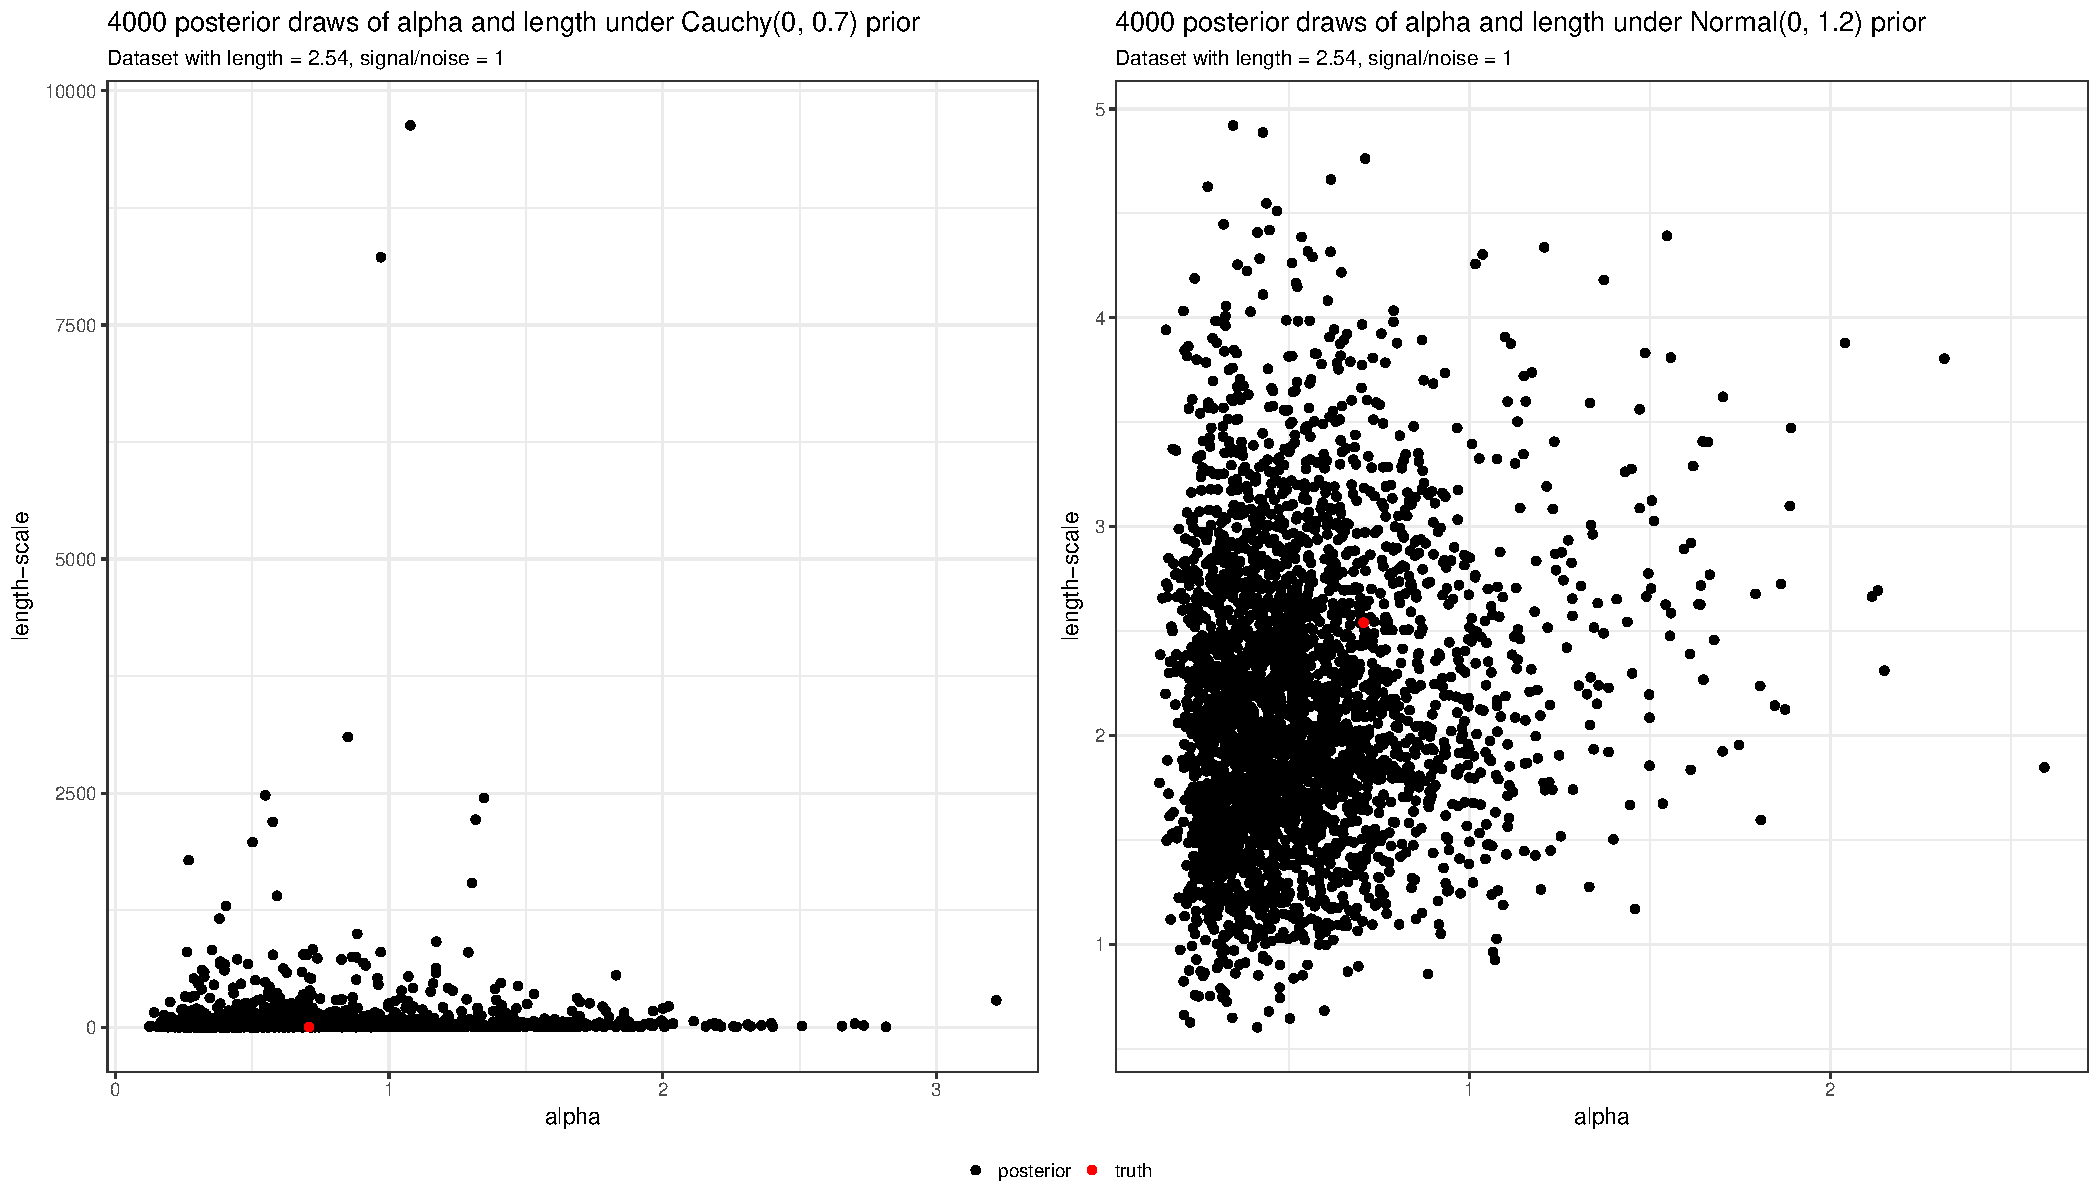
\includegraphics[width=\textwidth]{plots/dset_3_length_alpha.pdf}}
  \caption{Posterior distributions for $\ell$ and $\alpha$ under
  $\text{Half-Cauchy}(0, 0.7)$ and $\text{Half-Normal}(0, 1.2)$ priors for $\ell$} \label{gp_set_3_len}
\end{figure}

\begin{figure}[t]
  \centering
  \makebox[\textwidth]{\includegraphics[width=\textwidth, height=75mm]{plots/half_cauchy_dset_3_post_pred_mean.pdf}}
  \caption{4000 draws from the distribution of the posterior predictive means for new data over the $[-2,2]$ domain} \label{gp_set_3_post_pred_cauchy}
\end{figure}

Given that the $\text{Half-Cauchy}(0, 0.7)$ has a heavy tail, and given that
constant GPs and GPs that are near-constant can be very hard to distinguish
using any one data set, we recommend against using the Cauchy when there are
clear practical upper bounds to $\ell$. The heavy tail of the Cauchy puts too
much mass on data generating processes that are indistinguishable from one
another using finite data sets.

This can be seen in the distribution of posterior means for $\ell$ and $\alpha$
across simulations in the low signal-to-noise, large $\ell$ scenario in figure \ref{joint_len_alpha}. 

\begin{figure}[h]
  \centering
  \makebox[\textwidth]{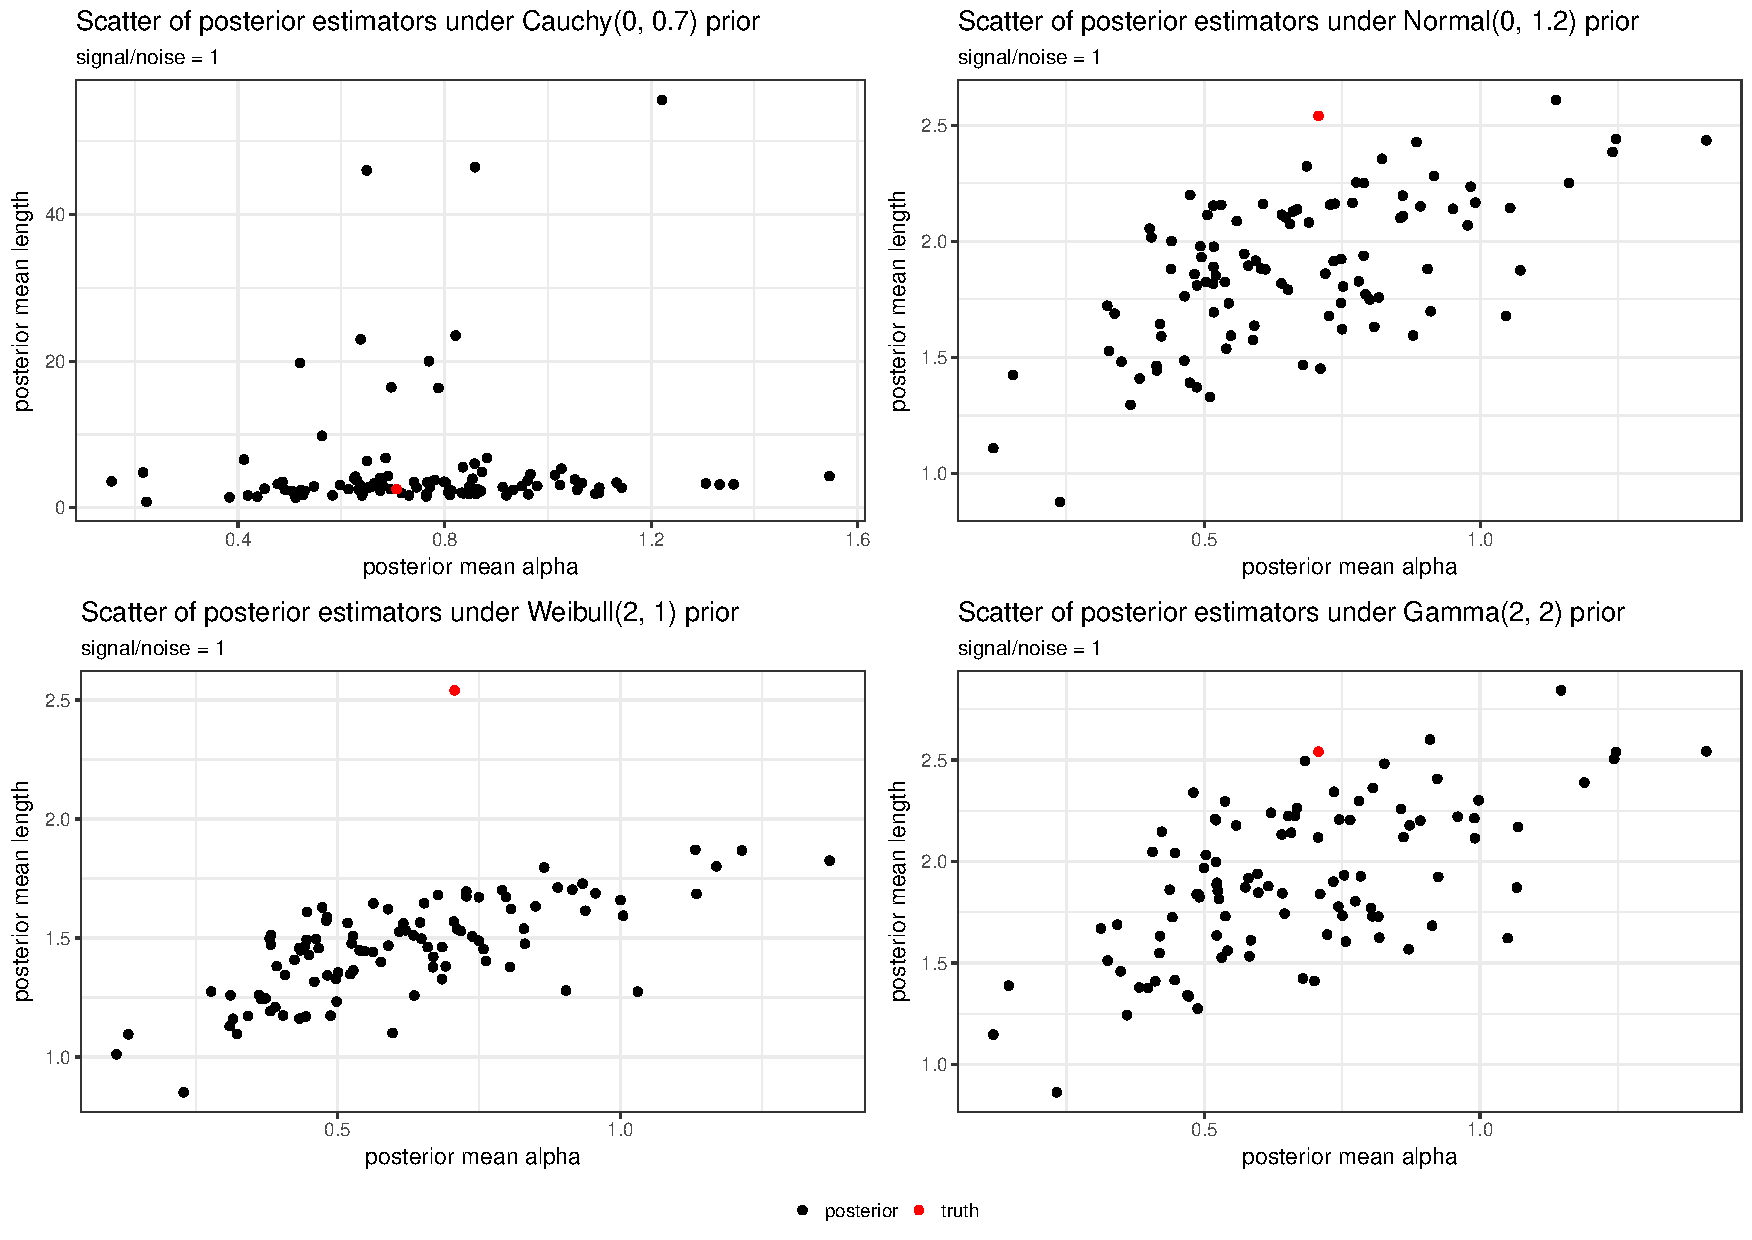
\includegraphics[width=\textwidth]{plots/dsets_2_5_alpha_0_7_alpha_length.pdf}}
  \caption{Posterior means of $\alpha$ and $\ell$. Data generated from GP with $\ell = 2.54, \alpha = 0.71, \delta = 0.71$.} \label{joint_len_alpha}
\end{figure}

We can see the fat tails of the Half-Cauchy leading to positively biased
estimates of length-scale in figure \ref{joint_len_alpha}. Given the paucity of
information in the data about the underlying mean function, our priors affect
the posterior mean estimates for $\ell$. This underscores the importance of
choosing weakly informative priors well. While the $\text{Half-Cauchy}(0, 0.7)$
allows for too much mass in the tail of the distribution, the
$\text{Weibull}(2, 1)$ has tails that are much too thin for the data generating
process, leading to estimates for length-scale that are negatively biased.

On the contrary, under the data generating processes that has a length-scale of
0.04 (with $\Exp{C_u | \alpha, \ell} = 31.62)$) and SN of 1, the posterior
means for $\ell$ are well-estimated by all priors, as can be seen in
\ref{joint_len_alpha_high_SN}. We had expected that priors with significant
mass near zero would have a hard time distinguishing between a length-scale of
zero and a length-scale greater than zero. However, this is likely a function
of the data being dense in $x$. We do see strong positive correlation between
$\ell$ and $\alpha$ in figure \ref{joint_len_alpha_high_SN}, which is a
byproduct of weak identifiability in the GP prior.

\begin{figure}[h]
  \centering
  \makebox[\textwidth]{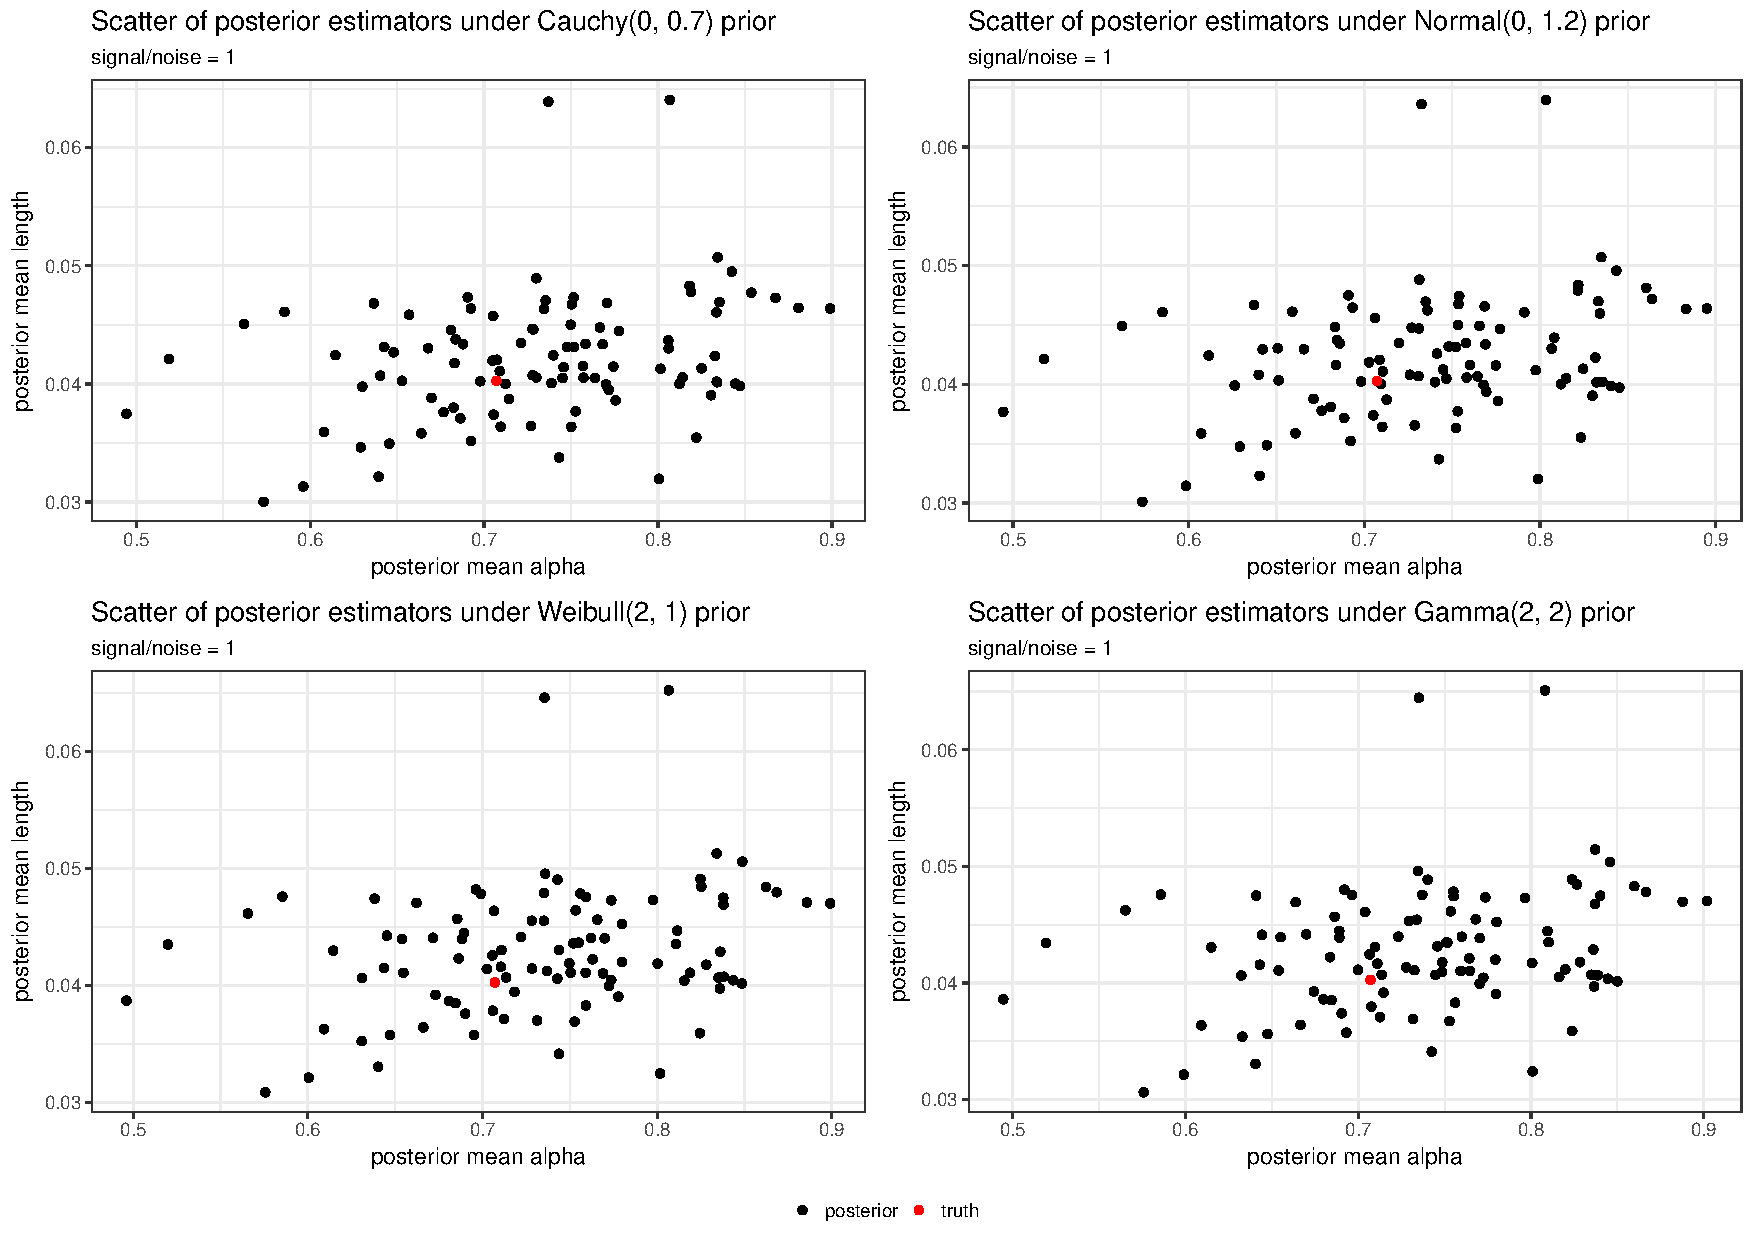
\includegraphics[width=\textwidth]{plots/dsets_0_05_alpha_0_7_alpha_length.pdf}}
  \caption{Posterior means of $\alpha$ and $\ell$. Data generated from GP with $\ell = 0.04, \alpha = 0.71, \delta = 0.71$.} \label{joint_len_alpha_high_SN}
\end{figure}

We present tables for summary statistics from the experiments across the 100
replicated datsets. We computed the 50\% and 90\% interval coverage, the bias,
the root mean squared error, and the mean interval width for $\alpha$ and
$\ell$. The most important takeaway is that if the tails of our priors are not
constructed with thought about the problem at hand, we can have low coverage,
or high bias, no matter the prior we use. We recommend a normal distribution
with care given to the scale of the process.

Another way to think about how to set priors on length-scale is to consider
the effective parameters 

These experiments suggest that setting a soft upper bound on $\ell$ with a
prior with a fast-decaying tail is a good weakly informative prior. More work
needs to be done to understand joint priors over $\alpha$, $\delta$, and
$\ell$.

\pagebreak

\section{Appendix}

\subsection{Stan code}

\begin{verbatim}
data {
  int<lower=1> D;
  int<lower=1> N;
  int<lower=1> N_pred;
  real x[N];
  vector[N] y;
  real x_pred[N_pred];
}
transformed data {
  vector[N] mu;
  matrix[N_pred, N_pred] nug_pred;

  mu = rep_vector(0, N);
  nug_pred = diag_matrix(rep_vector(1e-5,N_pred));
}
parameters {
  real<lower=0> length;
  real<lower=0> alpha;
  real<lower=0> delta;
}
model {
  matrix[N, N] L_Sigma;
  {
    matrix[N, N] Sigma;
    Sigma = cov_exp_quad(x, alpha, length);
    for (n in 1:N)
      Sigma[n, n] = Sigma[n,n] + square(delta);
    L_Sigma = cholesky_decompose(Sigma);
  }
  length ~ gamma(2, 2);
  delta ~ normal(0, 1);
  alpha ~ normal(0, 1);

  y ~ multi_normal_cholesky(mu, L_Sigma);
}
generated quantities {
  vector[N_pred] f_pred;

  {
    matrix[N, N] L_Sigma;
    vector[N] K_div_y;
    matrix[N, N_pred] k_x_x_pred;
    matrix[N, N_pred] v_pred;
    matrix[N_pred, N_pred] cov_f_pred;
    {
      matrix[N, N] Sigma;
      Sigma = cov_exp_quad(x, alpha, length);
      for (n in 1:N)
        Sigma[n, n] = Sigma[n,n] + square(delta);
      L_Sigma = cholesky_decompose(Sigma);
    }
    K_div_y = mdivide_left_tri_low(L_Sigma, y);
    K_div_y = mdivide_right_tri_low(K_div_y',L_Sigma)';
    k_x_x_pred = cov_exp_quad(x, x_pred, alpha, length);
    f_pred = k_x_x_pred' * K_div_y; 
    v_pred = mdivide_left_tri_low(L_Sigma, k_x_x_pred);
    cov_f_pred = cov_exp_quad(x_pred, alpha, length) - v_pred' * v_pred;

    f_pred = multi_normal_rng(f_pred, cov_f_pred + nug_pred);
  }
}
\end{verbatim}


\bibliographystyle{plainnat}
\bibliography{bib_inf_priors}

\end{document}
